\documentclass[9pt,twocolumn,twoside]{../../styles/osajnl}
\usepackage{fancyvrb}
\usepackage{hyperref}
\journal{i524} 

\title{Robot Operating System (ROS): A Useful Overview}

\author[1]{Matthew Lawson}

\affil[1]{School of Informatics and Computing, Bloomington, IN 47408, U.S.A.}

\affil[*]{Corresponding authors: laszewski@gmail.com}

\dates{paper2, \today}

\ociscodes{Cloud, I524, robot, ros, ROS}

% replace this with your url in github/gitlab
\doi{\url{https://github.com/eunosm3/classes/blob/master/docs/source/format/report/report.pdf}}


\begin{abstract}
The Open Source Robotics Foundation (OSRF) oversees the maintenance and development of the Robot Operating System (ROS).  ROS provides an open-source, extensible framework upon which roboticists can build simple or highly complex operating programs for robots.  Features to highlight include: a) ROS' well-developed, standardized intra-robot communication system; b) its sufficiently-large set of programming tools; c) its C++ and Python APIs; and, d) its extensive library of third-party packages to address a large proportion of roboticists software needs.  The OSRF distributes ROS under the BSD-3 license.
\newline
\end{abstract}

\setboolean{displaycopyright}{true}

\begin{document}

\maketitle

\section{Robot Operating System (ROS)}

\begin{figure*}[htbp]
\centering
\fbox{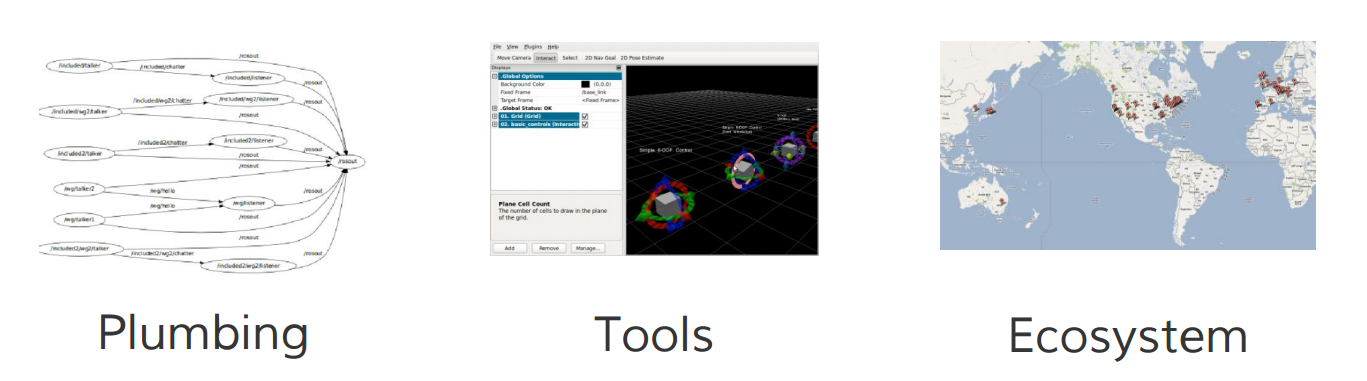
\includegraphics[width=\linewidth]{images/ros-is.png}}
\caption{A Conceptualization of What ROS, the \textit{R}obot \textit{O}perating \textit{S}ystem, Offers to Roboticists \cite{www-ros-ros-is}}
\label{fig:rosOverview}
\end{figure*}

\paragraph{1. Introduction}

The Open Source Robotics Foundation's middleware product \textit{Robot Operating System}, or ROS, provides a framework for writing operating systems for robots.  ROS offers "a collection of tools, libraries, and conventions [meant to] simplify the task of creating complex and robust robot behavior across a wide variety of robotic platforms" \cite{www-ros-about}. The Open Source Robotics Foundation, hereinafter OSRF or the Foundation, attempts to meet the aforementioned objective by implementing ROS as a modular system.  That is, ROS offers a core set of features, such as inter-process communication, that work with or without pre-existing, self-contained components for other tasks.

\paragraph{2. Architecture} 

The OSRF designed ROS as a distributed, modular system.  The OSRF maintains a subset of essential features for ROS, i.e., the core functions upon which higher-level packages build, to provide an extensible platform for other roboticists.  The Foundation also coordinates the maintenance and distribution of a vast array of ROS add-ons, referred to as modules.  Figure 1 illustrates the ROS universe in three parts: a) the plumbing, ROS' communications infrastructure; b) the tools, such as ROS' visualization capabilities or its hardware drivers; and c) ROS' ecosystem, which represents ROS' core developers and maintainers, its contributors and its user base.

The modules or packages, which are analogous to packages in Linux repositories or libraries in other software distributions such as \textit{R}, provide solutions for numerous robot-related challenges.  General categories include a) drivers, such as sensor and actuator interfaces; b) platforms, for steering and image processing, etc.; c) algorithms, for task planning and obstacle avoidance; and, d) user interfaces, such as tele-operation and sensor data display. \cite{www-software-categories}

\subparagraph{Communications Infrastructure || General}
OSRF maintains three distinct communication methods for ROS: a) \textit{message passing}; b) \textit{services}; and, c) \textit{actions}.  Each method utilizes ROS' standard communication type, the \textit{message} \cite{www-ros-core-components}.  Messages, in turn, adhere to ROS' \textit{interface description language}, or IDL. The IDL dictates that messages should be in the form of a data structure comprised of typed fields \cite{www-ros-messages}. Finally, \textit{.msg} files store the structure of messages published by various nodes so that ROS' internal systems can generate source code automatically.

\subparagraph{Communications Infrastructure || Message Passing}
ROS implements a publish-subscribe anonymous message passing system for inter-process communication, hereinafter pubsub, as its most-basic solution for roboticists.  A pubsub system consists of two complementary pieces: a) a device, node or process, hereinafter node, publishing messages, i.e., information, to a \textit{topic}; and b) another node \textit{listening to} and ingesting the information from the associated topic.  Pubsub's method of operation analogizes to terrestrial radio.  In the analogy, the radio station represents the publishing node, the radio receiver maps to the subscribing node and the frequency on which one transmits and the other receives represents the topic.  

The OSRF touts the pubsub communications paradigm as the ideal method  primarily due to its anonymity and its requirement to communicate using its message format.  With respect to the first point, the nodes involved in bilateral or multilateral conversations need only know the topic on which to publish or subscribe in order to communicate.  As a result, nodes can be replaced, substituted or upgraded without changing a single line of code or reconfiguring the software in any manner.  The subscriber node can even be deleted entirely without affecting any aspect of the robot except those nodes that depend on the deleted node.

In addition, ROS' pubsub requires well-defined interfaces between nodes in order to succeed.  For instance, if a node publishes a message without a crucial piece information a subscribing node requires or in an unexpected format, the message would be useless.  Alternatively, it would be pointless for an audio processing node to subscribe to a node publishing lidar data.  Therefore, a message's structure must be well-defined and available for reference as needed in order to ensure compatibility between publisher and subscriber nodes.  As a result, ROS has a modular communication system.  That is, a subscriber node may use all or only parts of a publishing node's message.  Further, the subscribing node can combine the data with information from another node before publishing the combined information to a different topic altogether for a third node's use.  At the same time, a fourth and fifth node could subscribe to the original topic for each node's respective purpose.  

Finally, ROS' pubsub can natively replay messages by saving them as files.  Since a subscriber node processes messages received irrespective of the message's source, publishing a saved message from a subscriber node at a later time works just as well as an actual topic feed.  One use of asynchronous messaging: postmortem analysis and debugging.

\subparagraph{Communications Infrastructure || Services}
ROS also provides a synchronous, real-time communication tool under the moniker \textit{services} \cite{www-ros-services}. Services allow a subscribing node to request information from a publishing node instead of passively receiving whatever the publishing node broadcasts whenever it broadcasts it.  A service consists of two messages, the request and the reply.  It otherwise mirrors ROS' message passing function.  Finally, users can establish a continuous connection between nodes at the expense of service provider flexibility.

\subparagraph{Communications Infrastructure || Actions}
ROS \textit{actions} offer a more-advanced communication paradigm than either message passing or services \cite{www-ros-actionlib}.  Actions, which use the basic message structure from message passing, allow roboticists to create a request to accomplish some task, receive progress reports about the task completion process, receive task completion notifications and / or cancel the task request.  For example, the roboticist may create a task, or equivalently, initiate an action, for the robot to conduct a laser scan of the area.  The request would include the scan parameters, such as minimum scan angle, maximum scan angle and scan speed.  During the process, the node conducting the scan will regularly report back its progress, perhaps as a value representing the percent of the scan completed, before returning the results of the scan, which should be a point cloud.

\subparagraph{Tools || Standard Messages}
ROS' extensive use in the robotics realm has allowed it to create message standards for various robot components \cite{www-ros-core-components}.  Standard message definitions exist "for geometric concepts like poses, transforms, and vectors; for sensors like cameras, IMUs and lasers; and for navigation data like odometry, paths, and maps; among many others."  These standards facilitate interoperability amongst robot components as well as easing development efforts by roboticists. 

\subparagraph{Tools || Robot Geometry Library}
Robots with independently movable components, such as appendages (with joints) or movable sensors, must be able to coordinate such movements in order to be usable.  Maintaining an accurate record of where a movable component is in relation to the rest of the robot presents a significant challenge in robotics \cite{www-ros-core-components}. 

\begin{figure}[htbp]
\centering
\fbox{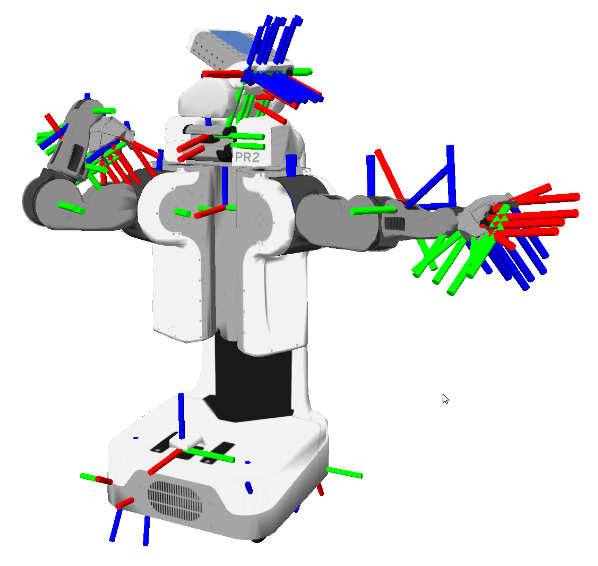
\includegraphics[width=\linewidth]{images/robotgeometry.png}}
\caption{A Simulated Robot with Many Coordinate Frames \cite{www-ros-robot-geometry}}
\label{fig:robotgeometry}
\end{figure}

ROS addresses this issue with its \textit{transform} library.  The \textit{tf} library tracks components of a robot using three-dimensional coordinate frames \cite{www-ros-robot-geometry}.  It records the relationship between coordinate frame positional values at sequential points in time in a tree structure.  tf's built-in functions allow the roboticist to transform a particular coordinate frame's values to same basis as a different coordinate frame's values.  As a result, the user, or the user's program, can always calculate any coordinate frame's relative position to any or all of the other coordinate frame positions at any point in time.  Although the first-generation library, \textit{tf}, has been deprecated in favor of the second-generation one, \textit{tf2}, the Foundation and ROS users still refer to the library as tf.

\subparagraph{Tools || Robot Description Language}
ROS describes robots in a machine-readable format using its \textit{Unified Robot Description Format}, or URDF \cite{www-ros-core-components}.  The file delineates the physical properties of the robot in XML format.  URDF files enable use of the tf library, useful visualizations of the robot and the use of the robot in simulations.  

\subparagraph{Tools || Diagnostics}
ROS' diagnostics meta-package, i.e., a package of related packages,  "contains tools for collecting, publishing, analyzing and viewing diagnostics data \cite{www-ros-diagnostics}."  ROS' diagnostics take advantage of the aforementioned message system to allow nodes to publish diagnostic information to the standard diagnostic topic.  The nodes use the diagnostic\_updater and self\_test packages to publish diagnostic information, while users can access the information using the rqt\_robot\_monitor package.  ROS does not require nodes to include certain information in their respective publications, but diagnostic publications generally provide some standard, basic information.  That information may include serial numbers, software versions, unique incident IDs, etc. 

\subparagraph{Tools || Command Line Interfaces (CLI)}

ROS provides at least 45 command line tools to the roboticist \cite{www-ros-cli}.  Therefore, ROS can be setup and run entirely from the command line.  However, the GUI interfaces remain more popular among the user-base.  Examples of ROS CLI tools include: a) \textit{rosmsg}, which allows the user to examine messages, including the data structure of .msg files \cite{www-ros-messages}; b) \textit{rosbag}, a tool to perform various operations on .bag files, i.e., saved node publications; and, c) \textit{rosbash}, which extends bash, a Linux shell program, with ROS-related commands. 

\subparagraph{Tools || Graphical User Interfaces (GUI)}
OSRF includes two commonly-used GUIs, \textit{rviz} and \textit{rqt} \cite{www-ros-core-components}, in the core ROS distribution.  rviz creates 3D visualizations of the robot, as well as the sensors and sensor data specified by the user.  This component renders the robot in 3D based on a user-supplied URDF document.  If the end-user wants or needs a different GUI, s/he can use rqt, a Qt-based GUI development framework.  It offers plug-ins for items such as: a) viewing layouts, like tabbed or split-screens; b) network graphing capabilities to visualize the robot's nodes; c) charting capabilities for numeric values; d) data logging displays; and, e) topic (communication) monitoring.   

\subparagraph{Ecosystem}
ROS benefits from a wide-ranging network of interested parties, including core developers, package contributors, hobbyists, researchers and for-profit ventures.  Although quantifiable use metrics for ROS remain scarce, ROS does have more than 3,000 software packages available from its community of users \cite{www-ros-why}, ranging from proof-of-concept algorithms to industrial-quality software drivers.  Corporate users include large organizations such as Bosch (Robert Bosch GmbH) and BMW AG, as well as smaller companies such as ClearPath Robotics, Inc. and Stanley Innovation.  University users include the Georgia Institute of Technology and the University of Arizona, among others \cite{www-ros-ecosystem}.  

\paragraph{3. API}

ROS supports robust application program interfaces, APIs, through libraries for C++ and Python.  It provides more-limited, and experimental, support for nodejs, Haskell and Mono / .NET programming languages, among others.  The latter library opens up use with C\# and Iron Python \cite{www-ros-api}.

\paragraph{4. Licensing}

The OSRF distributes the core of ROS under the standard, three-clause BSD license, hereinafter BSD-3 license.  The BSD-3 license belongs to a broader class of copyright licenses referred to as \textit{permissive licenses} because it imposes zero restrictions on the software's redistribution as long as the redistribution maintains the license's copyright notices and warranty disclaimers \cite{www-wikipedia-bsd}.

Other names for BSD-3 include: a) BSD-new; b) New BSD; c) revised BSD; d) The BSD License, the official name used by the Open Source Initiative; and, e) Modified BSD License, used by the Free Software Foundation.

Although the OSRF distributes the main ROS elements under the BSD-3 license, it does not require package contributors or end-users to adopt the same license.  As a result, full-fledged ROS programs may include other types of \textit{Free and Open-Source Software} \cite{www-wiki-foss}, or FOSS, licenses.  In addition, programs may depend on proprietary or unpublished drivers unavailable to the broader community.

\paragraph{5. Use Cases}
ROS' end-markets, its use cases, include manipulator robots, i.e., robotic arms with grasping units; mobile robots, such as autonomous, mobile platforms; autonomous cars; social robots; humanoid robots, unmanned / autonomous vehicles; and an assortment of other robots \cite{www-ros-ecosystem}.


\paragraph{5.1. Use Cases for Big Data}

Fetch Robotics, Inc. offers its \textit{Automated Data Collection Platform} robot to the market so corporations can "[g]ather environmental data more frequently and more accurately for [its] Internet of Things...and Big Data Applications. \cite{www-ros-fetch}" Fetch's system automatically collects data, such as RFID tracking (inventory management) or in-store shelf surveys. The latter service began in January 2017 when Fetch partnered with Trax Image Recognition, which makes image recognition software \cite{www-ros-trax}.  

\paragraph{6. Educational material}

Those interested in learning more about OSRF's ROS should visit ROS' homepage, \url{www.ros.org} or its wiki page, \url{wiki.ros.org}  In addition, ClearPath Robotics maintains a useful set of tutorials at \url{https://goo.gl/hRmM3k}.  Finally, several books dedicated to programming with ROS, such as \textit{Programming Robots with ROS: A Practical Introduction to the Robot Operating System} by Quibley, Gerkey and Smart can be purchased at retail.
\paragraph{7. Conclusion}

ROS offers a number of attractive features to its users, including a well-developed and standardized intra-robot communication system, modular design, vetted third-party additions and legitimacy via real-world applications.  Although its status as open source software precludes direct support from its parent organization, OSRF, for-profit organizations and the software's active community of users provide reassurances to any roboticist worried about encountering a seemingly-insurmountable problem.   

\paragraph{Acknowledgment}

I would like to thank my employer, Indiana Farm Bureau, for its support of my continuing education.

% \newpage

% Bibliography

\bibliography{references}
 
\section*{Author Biographies}
\begingroup
\setlength\intextsep{0pt}
\begin{minipage}[t][3.2cm][t]{1.0\columnwidth} % Adjust height [3.2cm] as required for separation of bio photos.
  \noindent
  {\bfseries Matthew Lawson} received his BSBA, Finance in 1999 from
  the University of Tennessee, Knoxville. His research interests include
  data analysis, visualization and behavioral finance.
\end{minipage}
\endgroup

\appendix

\section{Work Breakdown}

The work on this project was distributed as follows between the
authors:

\begin{description}

\item[Matthew Lawson.] Matthew researched and wrote all of the material for this paper.

\end{description}

\end{document}